\documentclass[10pt,twocolumn,letterpaper]{article}

\usepackage{cvpr_rebuttal}
\usepackage{times}
\usepackage{epsfig}
\usepackage{graphicx}
\usepackage{amsmath}
\usepackage{amssymb}

% Include other packages here, before hyperref.

% If you comment hyperref and then uncomment it, you should delete
% egpaper.aux before re-running latex.  (Or just hit 'q' on the first latex
% run, let it finish, and you should be clear).
\usepackage[pagebackref=true,breaklinks=true,letterpaper=true,colorlinks,bookmarks=false]{hyperref}

%%%%%%%%% PAPER ID  - PLEASE UPDATE
\def\cvprPaperID{89} % *** Enter the CVPR Paper ID here
\def\httilde{\mbox{\tt\raisebox{-.5ex}{\symbol{126}}}}
\setlength{\parindent}{0pt}

\usepackage{caption}

\begin{document}

%%%%%%%%% TITLE - PLEASE UPDATE
\title{Dynamic Probabilistic Linear Discriminant Analysis}  % **** Enter the paper title here

\maketitle
\thispagestyle{empty}


%%%%%%%%% BODY TEXT - ENTER YOUR RESPONSE BELOW
We thank Reviewers (R) 10 and 22 for their valuable feedback. R10 ("A good paper") and R22 ("The proposed methods are clearly derived from sound mathematical principles") are positive regarding the paper. R13 strongly rejects the paper (being very confident), even though it is evident that he/she is not knowledgeable at all regarding the field (probabilistic machine learning). We kindly request the assistance of the Area Chair on that.    %Note that in what follows, all citations correspond to references of the original paper submission. 


\textbf{[R10] Regarding Typos. }. Since, submission we have thoroughly edited the text to spot and correct all typos. An extended supplementary material will also accompany the paper (may it be accepted).  

\textbf{[R10] The authors should provide some experiments regarding the training time of the model}. Since, the methods scale linearly with regards to number of videos, frames, people etc. it is quite fast to train and test them. For example for the largest training set it takes few minutes to train (not more than 10 mins using un-optimised Matlab code). Testing, if carefully implemented, can be performed real-time. Detailed complexity evaluations will be included for each individual experimental setup. 

\textbf{[R10] The authors should consider comparisons of the proposed model with some other previous works like [20], [21].}. [20] is a CCA model that cannot be used for classification but for identifying shared structures. [21] proposes a unified view on probabilistic techniques. The only technique form [21] that is relevant is an alternative static PLDA which will include in the revised manuscript (performance very close to the tested static PLDA). 


% EFFECT OF CORRECTED FOREARM ANNOTATIONS
\textbf{[R13] How correlation are found if $\mathbf{A}=0.98\mathbf{I}$? If $A_{ij}$ very close to 1, how to differentiate $W_{ij}^t$ and $W_{ij}^{t+1}$? In Eq.(19), how to define the value of $A_{ij}$?}
First we would like to explain that $\mathbf{A}=0.98\mathbf{I}$ is used ONLY to PRODUCE artificial data in section 4.1 (a legitimate choice though, since it corresponds to a Slow feature dynamical system \cite{turner2007maximum}). In all experiments $\mathbf{A}_{ij}$ is found from the data through the application of the EM algorithm (standard practise, see 444-454). We refer the reviewer to standard textbooks \cite{bishop2006pattern} and tutorial papers \cite{roweis1999unifying} for further details on Linear Dynamical Systems (LDS). 


% HUMAN EFFORT COMPARED TO HUMAN ANNOTATION
\textbf{[R13] In Eq.(1), what the meaning of $\mathbf{y}_i$? There is no explanation in Section 2.1.. In Eq.(7), what is $Dy$ means? There is also no explanation in this section. etc.}
There is a clear explanation in 181-184 of the original paper. Unfortunately, we do not have space to describe in full detail standard models such as PPCA. Again we refer R13 to  \cite{bishop2006pattern,roweis1999unifying}. Equation (7) is a condensed form of equation (6) (it is easy to make the association between variables).


% building dense AAMs of patch-based AAMs with our pipeline cost 30 minutes for training with 600 images and fitting models cost the same time as normal AAM does. In our cases 5s for each fitting. Also, curve annotation requires much less effort, according to our experiment, putting landmarks on faces and ears requires 511s and 408s for each image including quality control, while only 42s and 38s need for annotating with curves.

% Manually annotating MPII (40K candidates), FLIC (20K+ candidates) require approximately 40K, 20K minutes correspondingly, while annotating using base line requires 700 minutes manually annotation + 40 minutes building time + 5s fitting time for each image. So 4K minutes and 2.3K minutes required for annotating entire MPII and FLIC dataset.



% FOCUS ON WRIST AND ELBOW
\textbf{[R13] Some state-of-the-art methods for YouTube face database, FERA database should also be compared in this section.} 
Comparisons exist in the original paper (please see 691-701 and 782-786). We will summarise them in a Table.


% ARE OUR LANDMARKS CONSIDERED GROUNDTRUTH
%\textbf{[R23] Can our landmarks be considered as groundtruth?} As shown in our %qualitative results (figure 7), our landmarks are, in most cases, much more %accurate than the existing landmarks. Figure~\ref{fig:noise_fitting} shows some %indicative results of fitting a model trained on our landmarks and on noisy %landmarks (crow. The results are very indicative of the impact that more accurate 5annotations could have to the effectiveness of an SDM.


% INITIALISATION OF FOREARM FITTING
\textbf{[R22]  The authors do not compare their techniques to any of the competing techniques that could be trained on the same data sets such as LBP, Convolutional Neural Networks or Support Vector Machines using Gabor filters or Gaussian Derivatives.}
The aim of the experiments were to show that our general machine learning methodology performs close to state-of-the-art even though combined with very simple features (IGO features).  Nevertheless, we compare with state-of-the-art techniques in 691-701 that use elaborate features.
Since, our method is a generic machine learning tool it can be used on top of arbitrary features (e.g. LBP and Gabor filters). For example we have now performed experiments using HoG and LBP features and the results have improved a lot. 

% LFPW EXPERIMENT
\textbf{[R23] Deep learning versus probabilistic methods.}
We agree with R23 that when a lot of data are available deep learning techniques can provide a good alternative. This is true for face recognition. But for facial expression recognition (FERA experiments) to the best of our knowledge there is no competing deep network proposed yet. We would like to note that DCNNs provide mainly good features which can be combined with any classification technique (including ours).

% PERFORMANCE ANALYSIS OF PROPOSED METHOD'S COMPONENTS
\textbf{[R22] There are very large data sets , such as the CASIA Webface data set (10,575 subjects and 494,414 images), that are available for deep learning techniques.} 
We agree that CASIA database is a valuable source of data (we will cite CASIA in the revised version). Nevertheless, it does not provide the amount of data necessary to match the performance of FaceNet by Google (200 Million) or DeepFace by FaceBook. 

% , as done with all software developed in our group,


\textbf{[R10-R25] Description of state-of-the-art (R25) and a table (R10).} We will include a table in the revised paper summarising all the state-of-the-art techniques, as well as further description in the text.

Finally, it goes without saying that all minor comments will be addressed. Also, we have already made steps towards making the code publicly available.




 %We plan to make such an analysis on a journal extension of this work. We refer the %Reviewer to the relevant bibliography of each component (SVS [39], NICP [3], Flow %[27], dAAM [2], patch AAM [52]).


%\begin{figure}[t!]
%    \centering
%    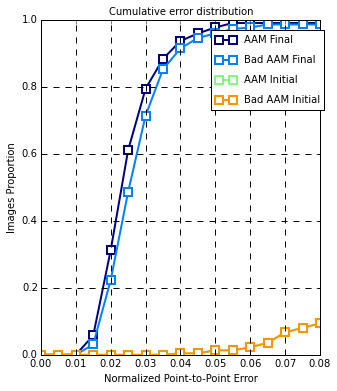
\includegraphics[width=0.48\columnwidth]{noise2}
%    \caption{Benchmark between AAM trained with consistant and noisy data}
%    \label{fig:noise}
%\end{figure}






% \textbf{[R23, R25] Effort of complete contour annotation of the forearm}. In the case of forearm, taking only two points into account actually requires slightly more effort. But for usecase that requires more points, our pipeline will be much faster. Moreover, contour annotation can work with semantic segmentation which can make the pipeline fully automatic (boundary of semantic segmentation gives contours needed).



% \textbf{[R23, R25] Manual effort spent on obtaining richer annotation worth ... SDM can be built with less effort does not seem to apply to the lower arm model ... }




{\small
\bibliographystyle{ieee}
\bibliography{egbib}
}

\end{document}
